\chapter{istar::USR: ultrafast shape recognition}

\section{Abstract}

Finding structurally similar compounds to a query ligand has been an important but daunting problem for a long time.

This is an ongoing collaborative project with Pedro J. Ballester from European Bioinformatics Institute, Cambridge, United Kingdom.

\section{Introduction}

Molecular shape has been widely acknowledged as a key factor for biological activity and thus is regarded as a very important pattern for which to search. Searching the molecular database for compounds that most closely resemble the shape of a given query molecule, be it a known inhibitor of a target protein, a natural product, or even a patented compound, finds pragmatic applications in ligand-based virtual screening \citep{1332,1380} and target fishing \citep{1407,1408,1402}. Therefore molecular similarity search assists in discovering structurally novel active compounds, or in identifying potential interacting target of bioactive ligands, which is useful for understanding the polypharmacology and safety profile of existing drugs. Furthermore, this approach can be applied to other scientific disciplines such as performing similarity comparisons between proteins or designing content-based Internet search engines for 3D geometrical objects \citep{1280}.

The molecular shape similarity can be quantified by methods based on structural alignment \citep{1440,887,1439} or shape recognition \citep{1379,1338,1331}. Structural alignment is also known as molecular superposition and requires precise geometric comparison which is often computationally intensive. Shape recognition, on the other hand, encodes shape information into a numerical feature vector, which can be subsequently used to compute a similarity score between two molecules very efficiently.% \citep{} Bioactive molecules: perfectly shaped for their target

USR (Ultrafast Shape Recognition) \citep{1379} was the very first non-superposition method for molecular shape comparison, and demonstrated superior computational performance at least three orders of magnitude faster than previously existing alignment-based methods. USR has another major advantage of being invariant to spatial rotation and translation, and hence circumvents the problematic requirement of aligning molecules. USR defines the shape of a molecule independently and for every molecule uses a fixed set of 12 descriptors derived from the first 3 statistical moments of distributions of interatomic distances between atoms and 4 purposely-selected centroids. The latter ensures that every molecule will have a unique location in the 12-dimensional chemical space spanned by the used descriptors, and consequently enables finding and visualizing clusters of molecules with similar shape \citep{1280,1332}. The ability of USR as a standalone method was studied to identify molecules sharing common biological activities through retrospective \citep{1332} and prospective \citep{1380} virtual screening experiments. USR was also used for deduplication in a virtual screening campaign \citep{1390} and in our iSyn \citep{1409,1387} \textit{de novo} ligand deisgn software.

Since USR was developed in 2007, there have been quite a few extensions \citep{1333,1436,1437,1334,1335,1337,1338,1331,1407,1408} to augment the method. \citep{1333} presented a hybrid approach composed of USR and the topological MACCS key descriptors, which are binary in nature and encode the presence or absence of 166 predefined structural fragments. It used the first four unbalanced moments of each distribution of atomic distances and incorporated additional chemical information through 2D structural similarity. Random Forest \citep{1310} was used for multi-class classification. Incorporating an additional central moment, the kurtosis, was found to significantly improved its performance. The addition of the fifth central moment, however, did not improve the performance sufficiently to justify the increased computational expense.

UFSRAT \citep{1436} addressed the lack of discrimination between compounds having similar shape but distinct pharmacophoric
features by subdividing atoms into four subsets which are heavy, hydrophobic, hydrogen bond acceptor or donor atoms, according to their atom types. For each subset, the four centroids were calculated, and so were the 12 USR descriptors. Therefore 48 descriptors were resulted. This was to ensure that similar compounds are able to make the same type of interactions within biological systems as the query ligand. UFSRAT is available as a web server at http://opus.bch.ed.ac.uk/ufsrat/. There are 28 databases to search against, with the largest one containing 4,853,000 conformers. UFSRAT is also employed for geometrical similarity searches in the EDULISS database \citep{1437} available at http://eduliss.bch.ed.ac.uk/ which comprises over 5 million commercially available compounds.

CSR \citep{1334} and USR:OptIso \citep{1335} attempted to tackle the lack of discrimination between chiral compounds. Their novel idea was to position the centroids in such a way that they clearly distinguishes between enantiomers, i.e. optical isomers. They both used cross product because it is an operator that transforms equivariantly under rotations and translations, but not under reflections. The two methods differed in selecting the centroids and in replacing or supplementing the new optical isomerism descriptor \citep{1335}. CSR \citep{1334} was tested on the DUD (Directory of Decoys) dataset \citep{87}, where a significant improvement in enrichment was found over USR. USR:OptIso \citep{1335} was shown to be helpful for analyzing molecules with stereogenic centers, atropisomerism, and in the clustering of conformers generated by systematic bond rotation.

ElectroShape \citep{1337,1338} extended the CSR \citep{1334} method by encoding electrostatics and liphophilicity through additional dimensions and centroids. In \citep{1337}, the partial charge was represented as a fourth coordinate, with atoms being identified by points in four-dimensional space. ElectroShape was validated using release 2 of the DUD dataset \citep{87}, and showed a near doubling in enrichment over USR and CSR. Different implementations of partial charge were also revealed to affect the enrichment performance significantly. The addition of a fourth statistical moment, as was done in \citep{1333}, improved USR and CSR but not ElectroShape, suggesting that adding extra information might not necessarily improve enrichment but could dilute the information already included. In \citep{1338}, ElectroShape was further extended by using atomic lipophilicity as an additional molecular property, with atoms being identified by points in five-dimensional space. This version of ElectroShape showed a clear improvement in performance, indicating that adding extra independent atomic properties makes shape-based enrichments even better.

USRCAT \citep{1331} extended the UFSRAT \citep{1436} method by identifying five subsets of atoms with the help of the SMARTS patterns used for atom typing in the CREDO database \citep{522}. The five subsets were chosen to be heavy, hydrophobic, aromatic, hydrogen bond acceptor or donor atoms. Aromaticity was added to USRCAT as a pharmacophoric subset because USR was unable to discriminate between long, chain-like molecules such as certain heteropeptides and long alkylchains in particular. Unlike UFSRAT \citep{1436}, USRCAT \citep{1331} derived the four centroids from heavy atom coordinates and used them to calculate the distributions for all the five subset moments to improve screening performance. USRCAT was shown to outperform the traditional USR method in a retrospective virtual screening benchmark with the DUD-E (Directory of Decoys, Enhanced) dataset \citep{1185}. The highest enrichment factors were only achieved if the LEC (Lowest Energy Conformer) of an active was used as a query and if the LECs were included in the target set, but this observation cannot be generalized. DUD-E was found to be not ideal to benchmark the virtual screening performance of global shape similarity algorithms such as USR and its variants due to the large variations in molecular size of the active ligands.

Another study \citep{1407} used a reference set of 224,412 molecules active on 1,700 human proteins and showed that accurate target prediction can be achieved by using a multiple logistic regression to combine different measures of chemical similarity based on both chemical structure and molecular shape, with the former using FP2 fingerprints and the latter using ElectroShape \citep{1338}. This hybrid method was later developed into the SwissTargetPrediction \citep{1408} web server, available at http://www.swisstargetprediction.ch/, to identify new targets for uncharacterized molecules or secondary targets for known molecules. With data collected from the ChEMBL database version 16 \citep{1441}, the molecular library was expanded to 280,000 compounds active on 2,686 targets of the organisms of human, mouse, rat, cow and horse. Mapping predictions by homology within and between different species, a powerful approach to translate results obtained in model organisms to human, were enabled for close paralogs and orthologs.

Among the USR variants mentioned above, only three of them \citep{1436,1437,1408} have been made available as web servers together with different databases for different purposes. The UFSRAT \citep{1436} and EDULISS \citep{1437} web servers both employ the UFSRAT \citep{1436} method for ligand similarity search. However, as pointed out in \citep{1331}, this method is incapable of discriminating between long, chain-like molecules such as certain heteropeptides and long alkylchains because aromaticity is not considered as a pharmacophoric subset; besides, calculating the four centroids for each set of atoms individually is problematic because either the parameters cannot be calculated at all or the underlying distance distributions are not with respect to the overall shape of a molecule and not meaningful when some pharmacophoric features are rarer than others. The UFSRAT \citep{1436} web server constrains the input query ligand to be one molecule in SDF format only, and implements no online visualization. The EDULISS \citep{1437} web server requires drawing a query structure in a Java molecular editor, which is being disabled on more and more systems due to security concerns. The SwissTargetPrediction \citep{1408} web server, on the other hand, comprises well-annotated active compounds and is primarily used for predicting the target proteins of bioactive small molecules but not for prospective virtual screening purposes.

In this project we aim to provide an istar-based \citep{1362} web server for large-scale prospective virtual screening using USR-like methods. We choose to employ USR \citep{1379} and USRCAT \citep{1331} because they have demonstrated pragmatic usefulness in prospective \citep{1380} and retrospective \citep{1331} virtual screening experiments, respectively, and their source code is freely available. Our istar::USR has several distinctive features. First, it uses both USR and USRCAT. Second, its database comprises 230 million low energy conformers of 23 million compounds collected from ZINC \cite{532,1178}. Third, it supports multiple query ligands in one job. Fourth, it utilizes three levels of parallelism to accelerate job execution.

\section{Methods}

\subsection{USR and USRCAT}

USR is based on the observation that the shape of a molecule is uniquely determined by the relative position of its atoms, which is in turn determined by the set of all interatomic distances. This convenient representation is independent of molecular orientation or position, and thus eliminates any need for alignment or translation. The interatomic distances are heavily constrained by the forces that hold the atoms together, and hence they contain more than sufficient information to accurately describe molecular shape. So it is possible to use a set of all atomic distances from a small number of strategic reference locations uniquely defined in every molecule and meanwhile retain the discriminative power necessary to distinguish between molecules.

The four reference locations are selected to be the molecular centroid (ctd), the closest atom to ctd (cst), the farthest atom to ctd (fct), and the farthest atom to fct (ftf). These locations represent the centre of the molecule and its extremes, and thus are well separated. In this way molecular shape is described by four distributions of atomic distances, where the number of atomic distances is proportional to the number of atoms. In order to compare molecules with different number of atoms, the first three moments of these distributions are computed and used to encode shape information instead. These moments have semantics indeed. For instance, the 1st, 2nd and 3rd moments of distribution of atomic distances to the molecular centroid (ctd) capture the size, variance and skewness of the molecule, respectively. Selecting the first three moments provides an excellent compromise between the efficiency and the effectiveness of the method. Finally the shape similarity score of two molecules is calculated through the sum of least absolute differences of their respective moments.

In this study the first three moments are computed in the same way as ElectroShape \citep{1337} does, which is slightly different than the way used in some other studies \citep{1379,1332,1380,1331}. Mathematically, for a distribution of atomic distances $\{d_i\}_{i=1}^n$ to a reference location, the first three moments are semantically the mean, the standard deviation, and the cube root of the third central moment, respectively. Their exact expressions are shown in equations \eqref{usr:moment1}, \eqref{usr:moment2} and \eqref{usr:moment3}. The roots are intended to provide all moments with linear space dimension in \AA, unlike the skewness, for instance, which is unitless. This computation allows the distributions to contain only one sample, in which case the 2nd and 3rd moments will be zeros.

\begin{equation}
m_1=\frac{1}{n}\sum_{i=1}^{n}{d_i}
\label{usr:moment1}
\end{equation}

\begin{equation}
m_2=\sqrt[2]{\frac{1}{n}\sum_{i=1}^{n}{(d_i-m_1)^2}}
\label{usr:moment2}
\end{equation}

\begin{equation}
m_3=\sqrt[3]{\frac{1}{n}\sum_{i=1}^{n}{(d_i-m_1)^3}}
\label{usr:moment3}
\end{equation}

Dimension reduction: any ligand structure is mapped to a point in a 12 dimensional space. In combination with a suitable clustering algorithm, one could find clusters in a molecular database in order to select the most representative molecule of each cluster. The latter could be applied, for example, as a way to avoid repeating expensive biological tests on similar molecules.  This opens the door to the application of existing clustering algorithms to find groups of similar molecules as a way to analyse the molecular diversity of a database in terms of molecular shape. \citep{1280,1332}

Dissimilarity transformed into a normalized similarity score. (Eq \ref{usr:usr}) Any inverse monotonic function can do.

\begin{equation}
S_{qi}=\frac{1}{1+\frac{1}{12}\sum_{l=1}^{12}|M_l^q-M_l^i|}
\label{usr:usr}
\end{equation}

USR is highly extensible: changing reference points \citep{1334,1335}, using higher orders of moments \citep{1333,1337}, using subsets of atoms \citep{1436,1331}.

USRCAT extends USR in the last approach. Atoms are partitions into five subsets. The five subsets were chosen to be heavy, hydrophobic, aromatic, hydrogen bond acceptor or donor atoms.% Their SMARTS patterns are respectively [!#1], [#6+0!\$(*~[#7,#8,F]),SH0+0v2,s+0,S^3,Cl+0,Br+0,I+0], [a], [\$([O,S;H1;v2]-[!\$(*=[O,N,P,S])]),\$([O,S;H0;v2]),\$([O,S;-]),\$([N\&v3;H1,H2]-[!\$(*=[O,N,P,S])]),\$([N;v3;H0]),\$([n,o,s;+0]),F], [N!H0v3,N!H0+v4,OH+0,SH+0,nH+0].
In the case of an empty subset, for examples if no hydrogen bond donors are found, then the corresponding elements in the moment vector will be set to zero.

When calculating similarity score between two molecules, the five subsets can be weighted. S=1/(1+w1S1+w2S2+...+w5S5). Update the equation with weights. equation 1 in {1331}.

\begin{equation}
S_{qi}=\frac{1}{1+\frac{1}{12}\sum_{l=1}^{12}|M_l^q-M_l^i|}
\label{usr:usrcat}
\end{equation}

\subsection{USR on istar}

It is necessary to include more than one conformer per compound in the database, since flexible molecules can adopt different shapes, and thus the more of these conformations that are included in the database, the less likely it is to miss molecules with the desired pattern. Could have an average of about 200 conformations per small organic molecules \citep{1332}, or up to 292 additional conformations \citep{1280}.

All Clean Subset from ZINC (N=23,129,083)
Large 3D database, ZINC \citep{532,1178}, istar \citep{1362}, 23 million.
Like in istar::idock, we used the same database, for prospective screening.

The final step for the generation of the test database is to calculate 3D molecular conformations for each of the considered 2D chemical structures. The conformers of a particular molecule are in general geometrically distinct and have low potential energy, as conformers with high internal energy are in principle less likely to occur in nature.

\begin{figure}
\centering
\subfloat[Positional degree of freedom.]
{
  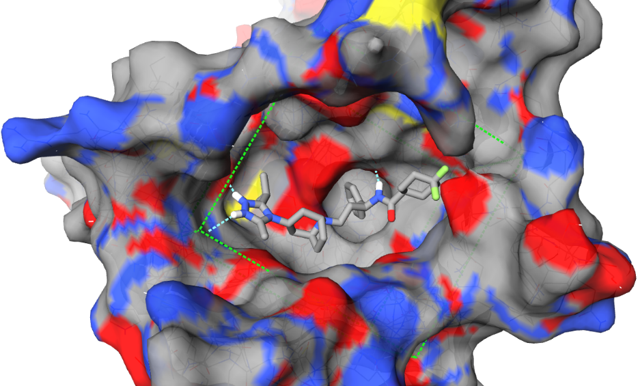
\includegraphics[width=0.48\linewidth]{../usrt/MRV0.png}
}
\subfloat[Orientational degree of freedom.]
{
  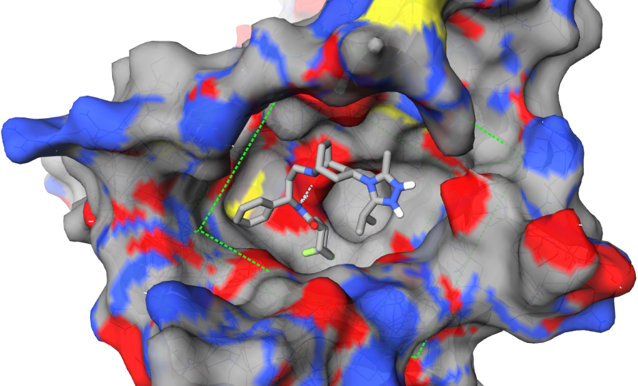
\includegraphics[width=0.48\linewidth]{../usrt/MRV1.png}
}
\caption{Two very different docked poses of the marketed HIV drug maraviroc in complex with the human CCR5 chemokine receptor (PDB: 4MBS). The protein is rendered in molecular surface representation. The ligand is rendered in stick representation. The binding cavity on the protein surface is depicted by a green cubic box. The putative intermolecular hydrogen bonds are shown as cyan dashed lines. The ligand poses were generated by idock \citep{1153} and the figure was rendered by iview \citep{1366}.}
\label{usr:MRV}
\end{figure}

There are numerous 2D-to-3D conversion tools: OMEGA \citep{462} or CORINA \citep{1392} or Cyndi \citep{1393,1394} or CONCORD \citep{}. \citep{1127} evaluated four of them: BALLOON, CONFAB, FROG2, and RDKIT, and concluded that RDKit performed the best. Therefore we will use RDKit to generate conformers. Also mention the C++ version rather than Python, and the constraints of not having a large RMSD. So postprocessing is required, as suggested in \citep{1127}.

Several levels of parallelism: multiple database ligands, multiple query ligands, multiple features.

Parallelized at the coarse grained level of a database of ligands to compare against.

AVX (Advanced Vector Extensions) instructions. Use PowerPoint to draw a diagram here to illustrate. unrolling, sub, abs, hadd.

Time analysis: t = n(tq+ts)

In UFSRAT \citep{1436}, the input format of query ligand is limited to SDF. We support SDF, MOL2, XYZ, PDB, PDBQT.

\section{Conclusions}

USR has advantages in being independent of position and orientation.

Emphasize computational efficiency, 3 orders of magnitude faster than ESshape3D, and applicable to large-scale ligand database like istar \citep{1362}, which has collected 23 million ligands from ZINC \citep{532,1178}.

the reason why a database is populated with multiple conformers of each flexible compound is to reduce the possibility of missing compounds with similar shape to the query.

\section{Availability}

istar::USR is free and open source under Apache License 2.0. It is available at http://istar.cse.cuhk.edu.hk/usr.

\section{Future works}

USR is independent of position and orientation, but is dependent on torsions. Nevertheless, none of the above variants are independent of torsions. We present USRT, the first algorithm that is invariant of torsions. In the following sections, we describe USR and USRT, their effectiveness and efficiency.

We present the first algorithm that can distinguish ligands with different torsions. We call it USRT (Ultrafast Shape Recognition with Torsions). In USRT, the reference atom is chosen to be the atom connecting to the parent frame. It is BRANCH X Y, and is often the first of the current frame. For the ROOT frame, it is the first atom.

Figure \ref{usr:T27} shows two conformations with different torsions. This is a rotatable bond. This branch can rotate along the rotatable bond and flip to the right hand side. A torsion is the rotating angle, so it is in the range of -$\pi$ to $\pi$. 

\begin{figure}
\minipage{0.5\textwidth}
\centering
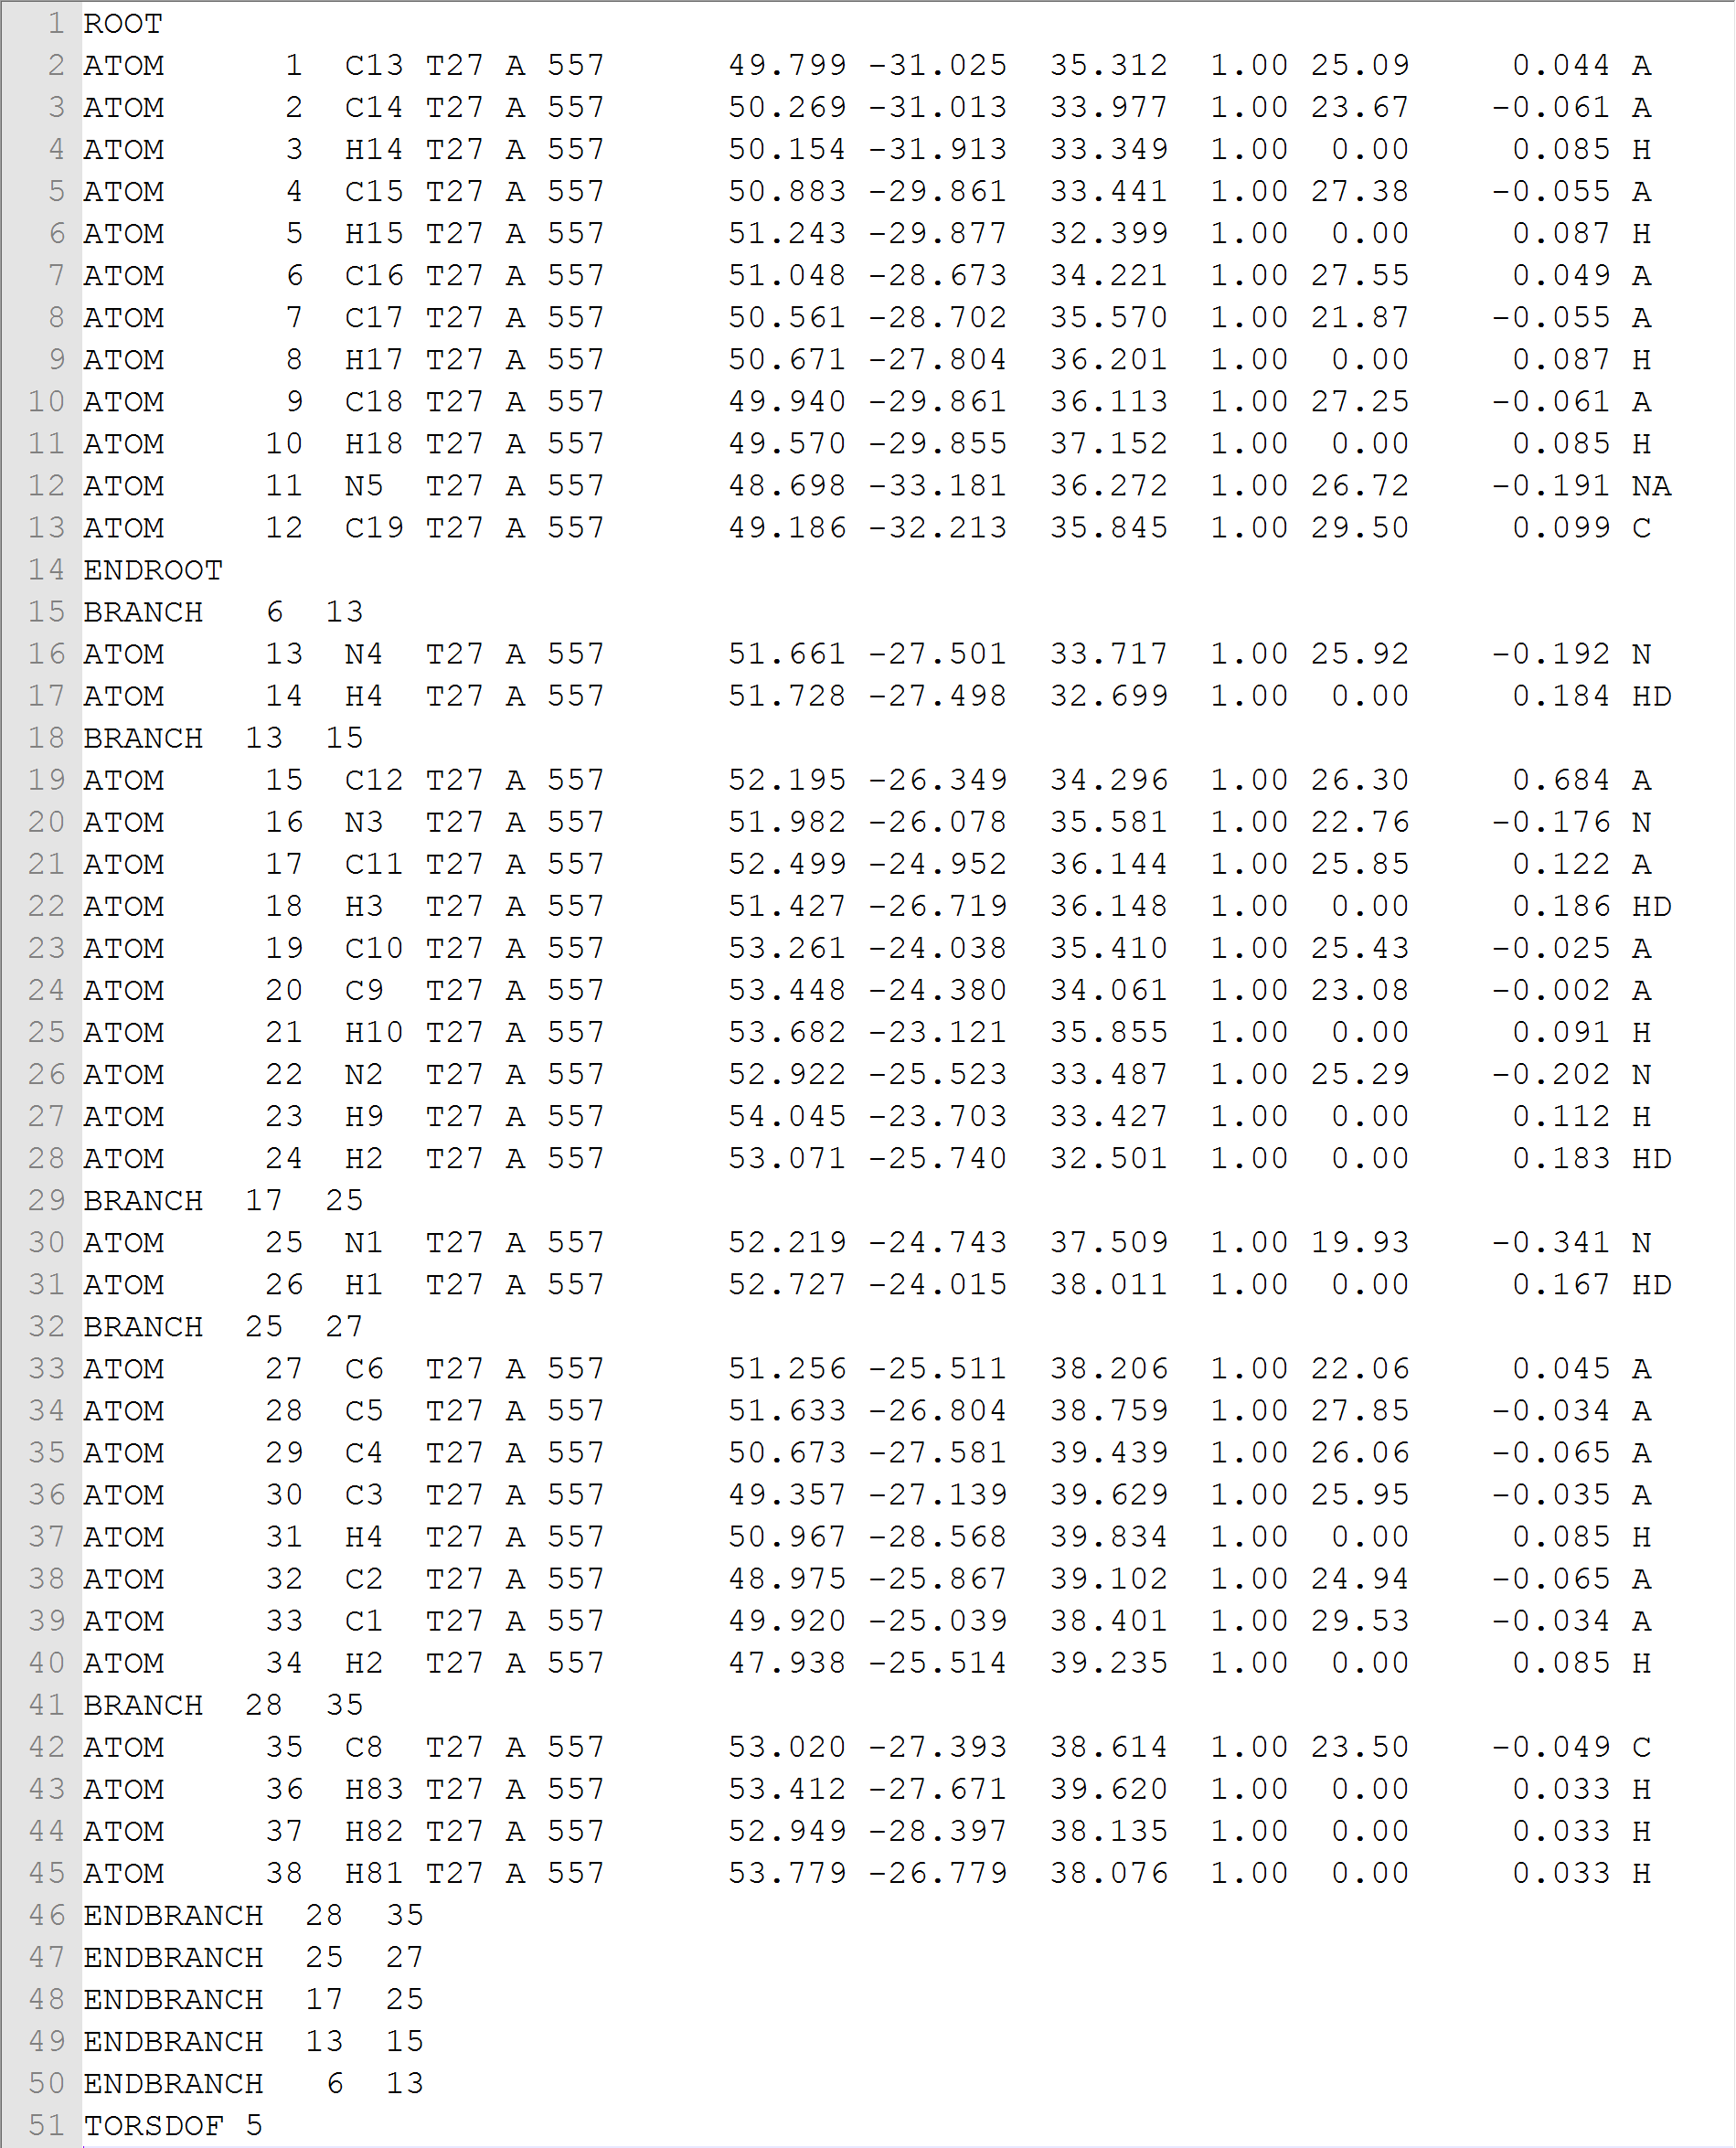
\includegraphics[width=1.36\textwidth,natwidth=1899,natheight=2350]{../usrt/T27CrystalPDBQT.png}
\endminipage
\minipage{0.5\textwidth}
\centering
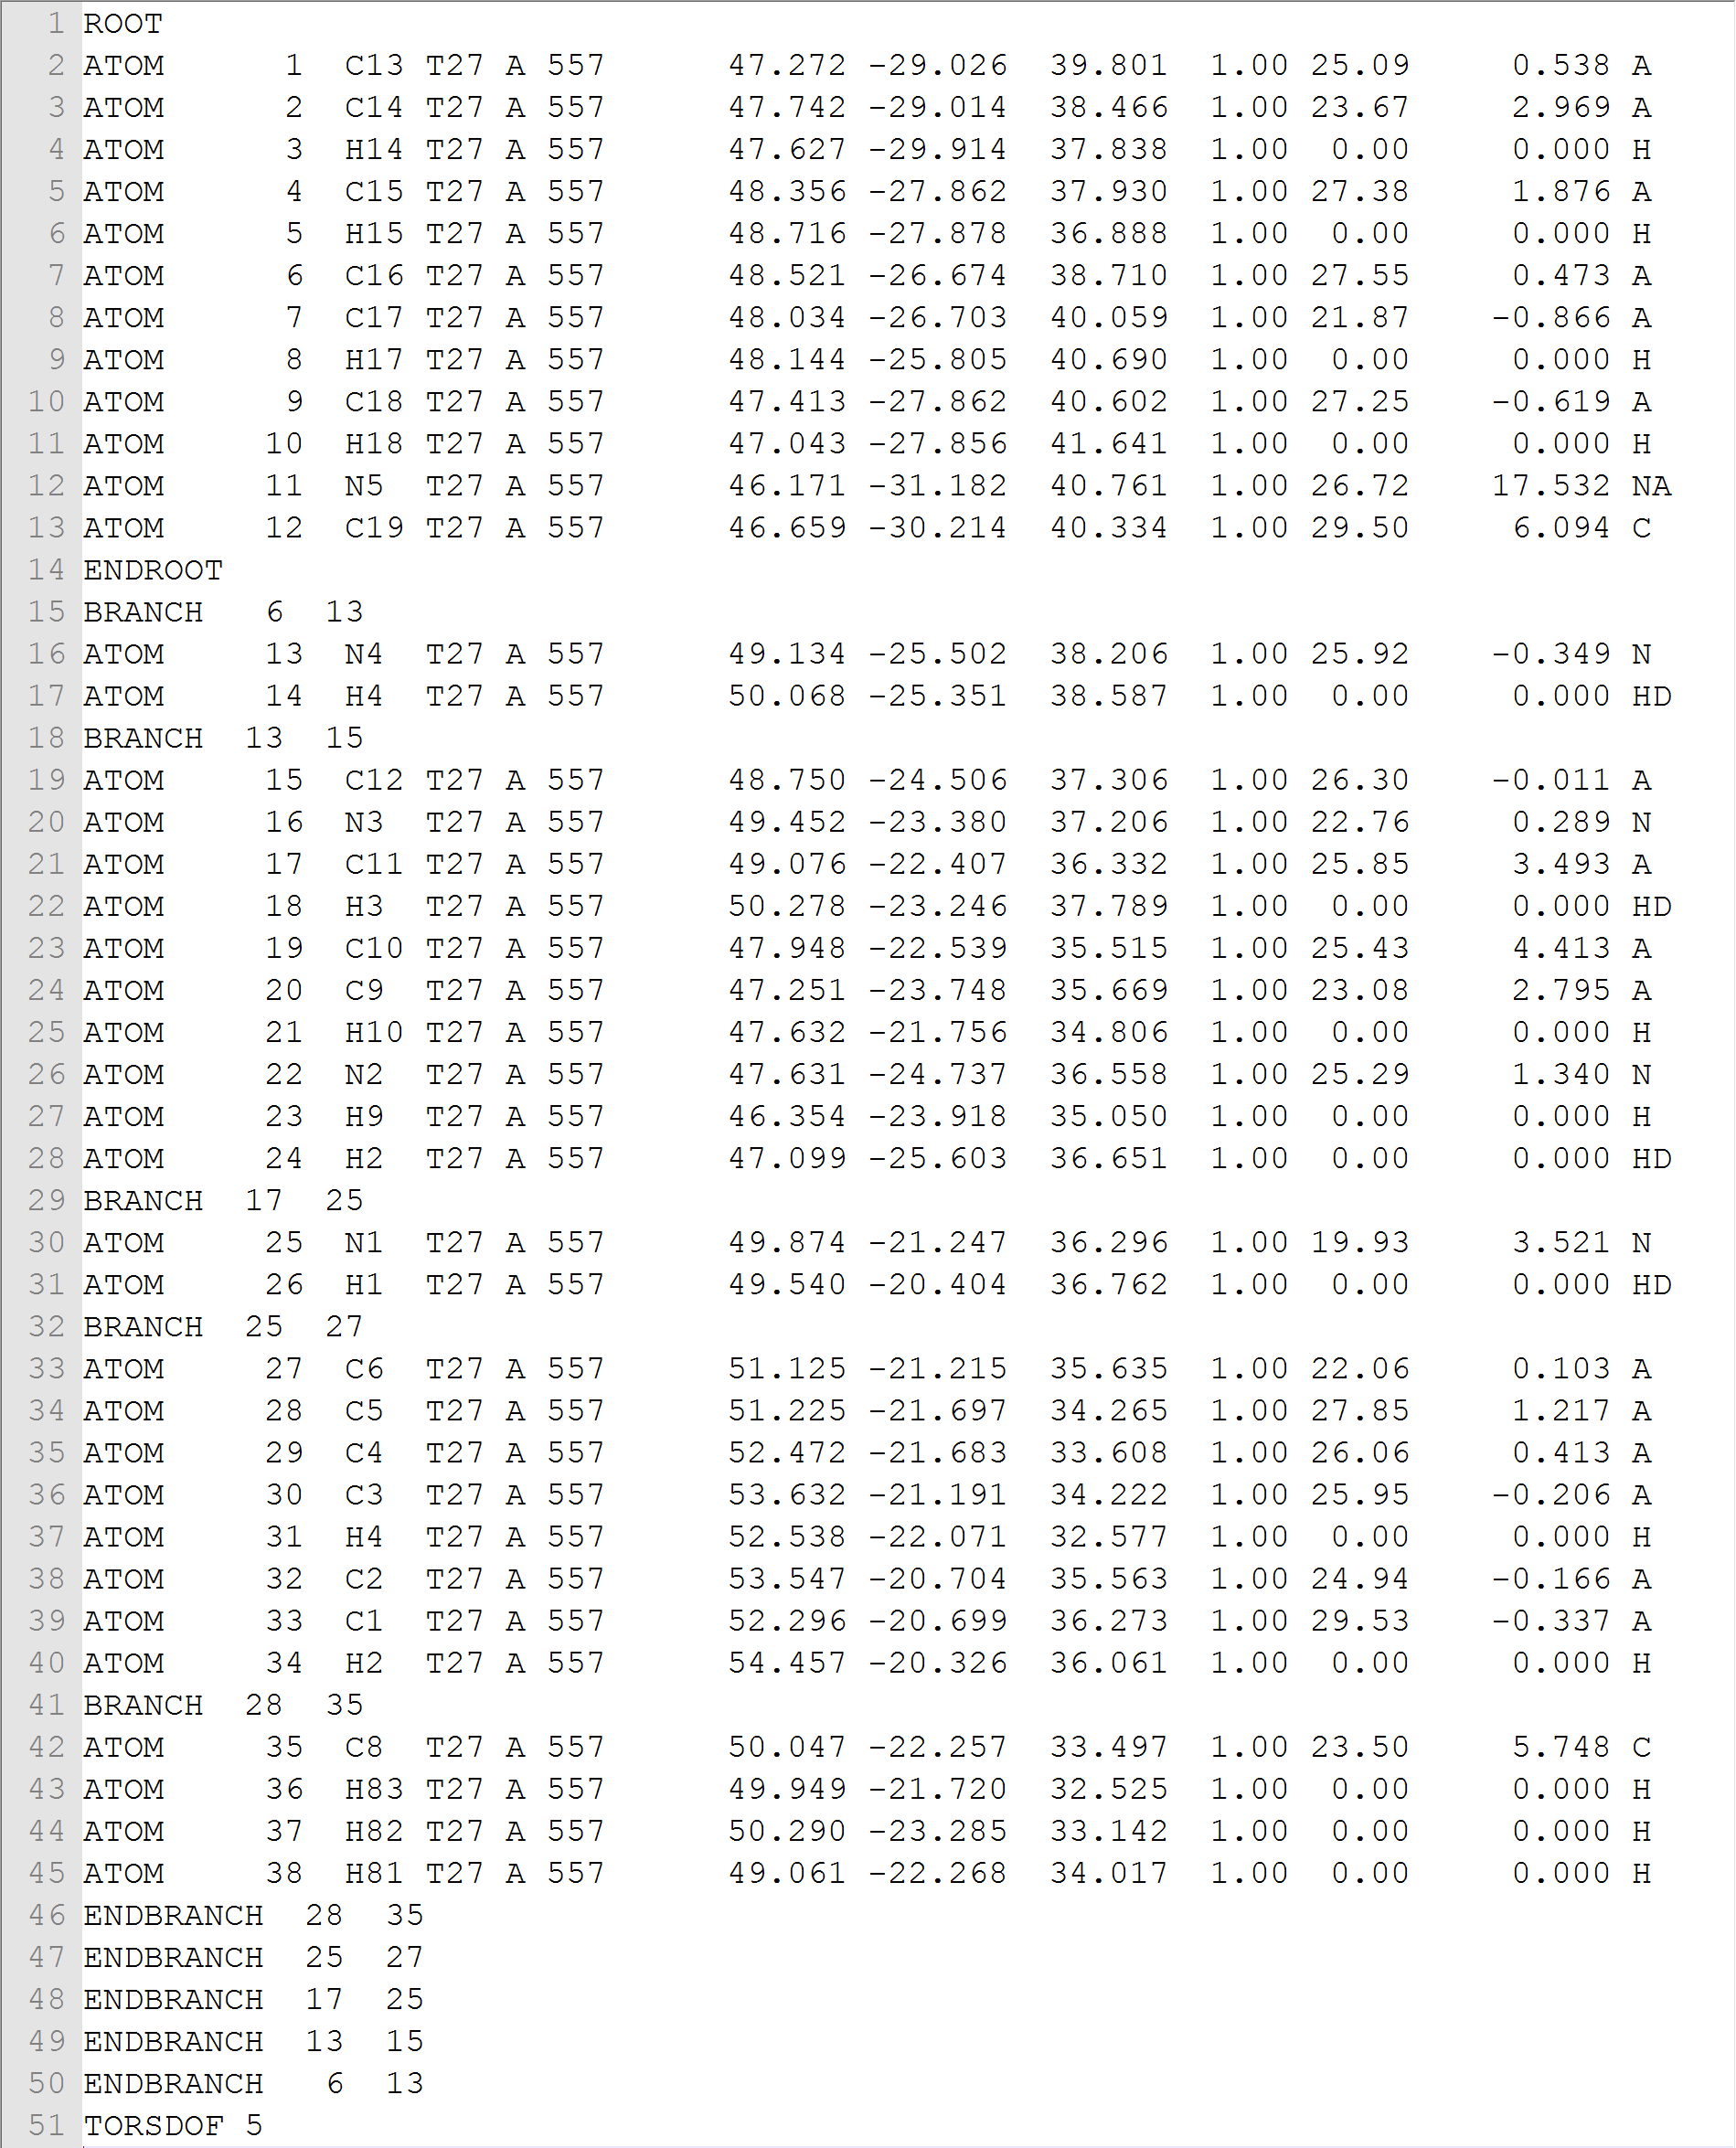
\includegraphics[width=1.36\textwidth,natwidth=1899,natheight=2350]{../usrt/T27DockedPDBQT.png}
\endminipage
\\
\minipage{0.5\textwidth}
\centering
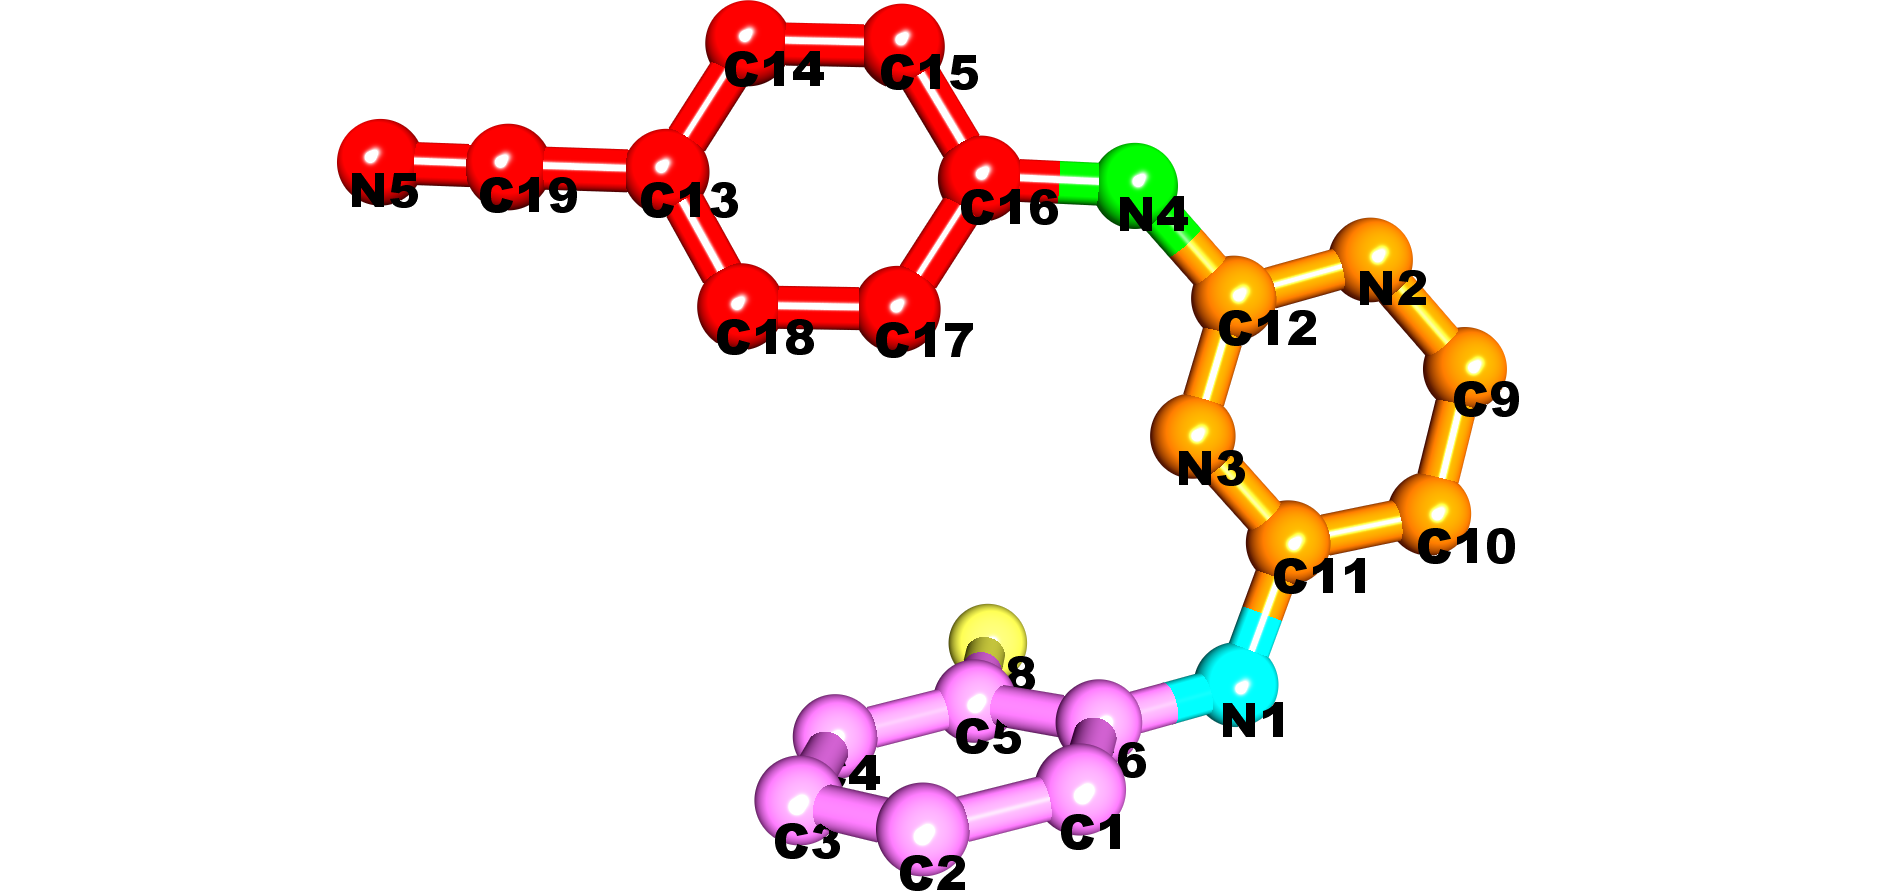
\includegraphics[width=1.36\textwidth,natwidth=1904,natheight=894]{../usrt/T27Crystal.png}
\endminipage
\minipage{0.5\textwidth}
\centering
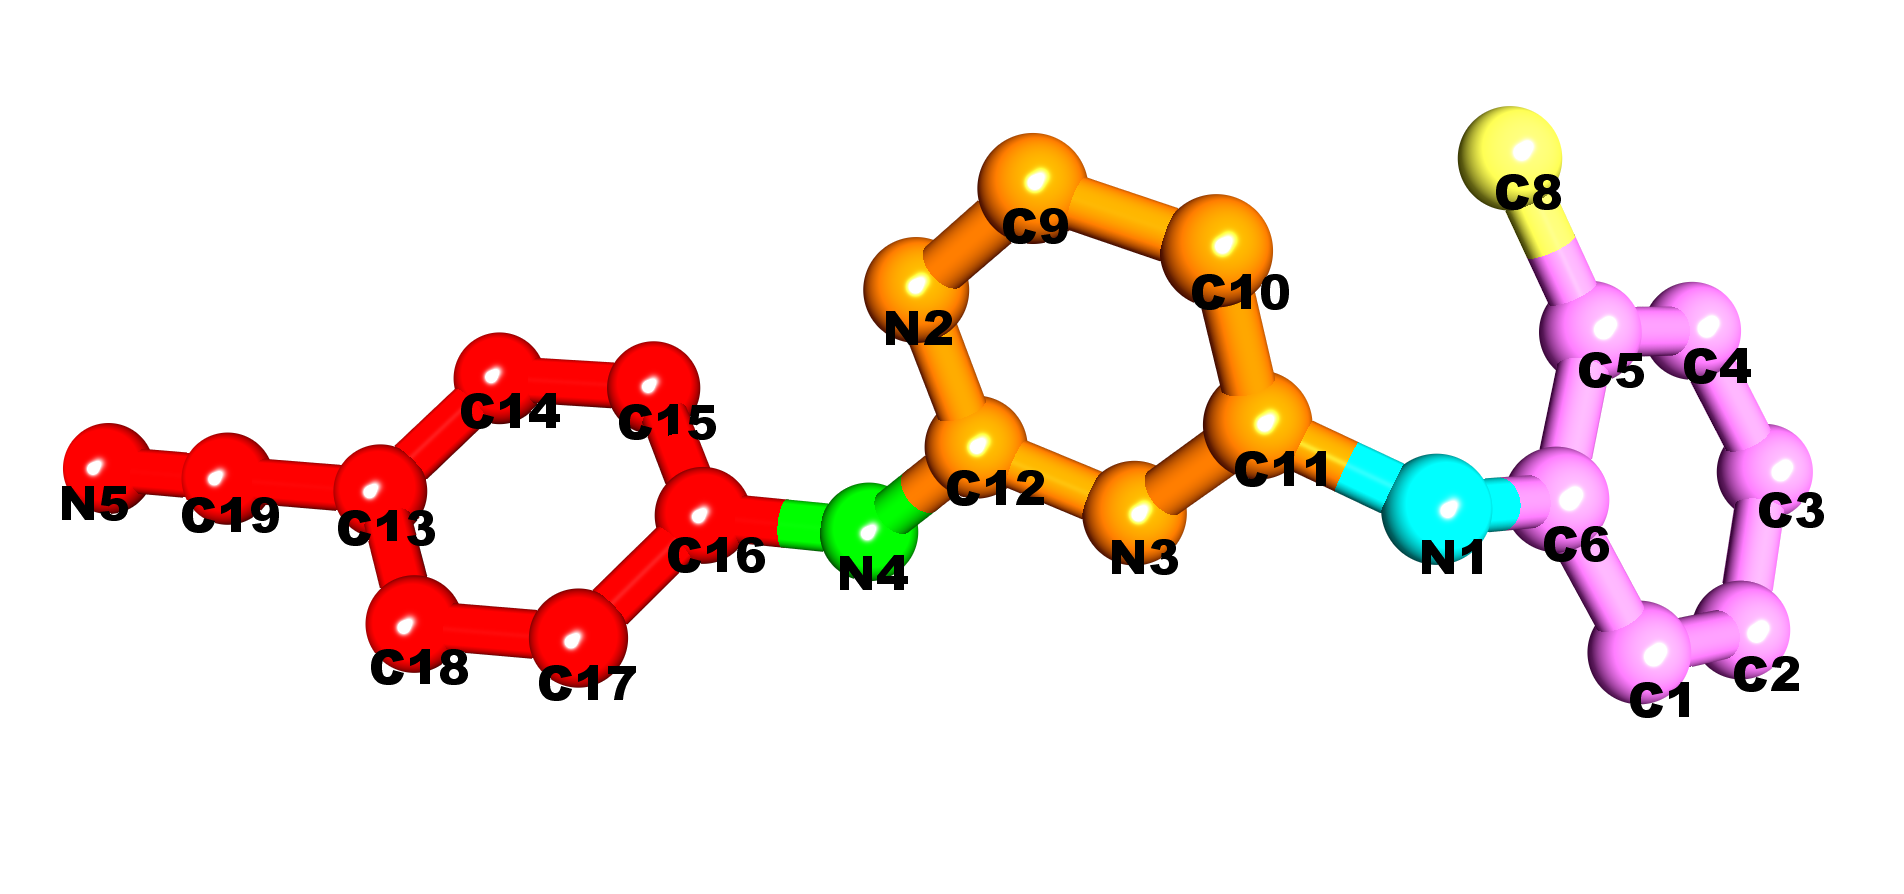
\includegraphics[width=1.36\textwidth,natwidth=1904,natheight=894]{../usrt/T27Docked.png}
\endminipage
\caption{Two very different poses of the same ligand, which has six frames and five rotatable bonds. Top row: the contents of the two poses in PDBQT format. Bottom row: the two poses in ball-and-stick representation. The atoms and bonds in the same frame are rendered in the same color.}
\label{usr:T27}
\end{figure}

Once a reference atom is determined, the next is to compute inter-atom distances and their 1st, 2nd, 3rd moments. The output of USRT is a feature vector, which maps to a point in a high dimensional space. The length of the feature vector depends on the number of rotatable bonds. This format a natural clustering: the ligands having the same number of rotatable bonds are first categorized, and then all existing clustering algorithms can be utilized.

USRT inherits advantages from USR, like being ultrafast and extensible. It circumvents the need of aligning the molecules before testing for similarity. Compatible with USRCAT \citep{1331}, USR+MACCS \citep{1333} and possibly other USR variants \citep{1334}. can combine with other USR variants, e.g. USRCAT.

USRT is a general method that can be applied to various drug design applications, including de novo ligand deduplication and clustering. No conformers are required. the unbound bioactive conformation could be in principle significantly different from the corresponding bound conformation. No more considerations of using bound or unbound conformations.

Although very promising, major problems are: tree structure output, child frame matching, known ROOT frame, in-frame atom types, connector atom types. This raises the obvious question of how to compare molecules with different number of torsions, which are introduced by flexible ligand docking. Frames with less than 2 heavy atoms are ignored or assigned zero. Could be inactive frames like -CH3, -NH2 or -OH. Cannot compute 2nd and 3rd moments. Can incorporate connecting atoms of child branches. We will address the above limitations in future research using dynamic programming with frame insertion/deletion.

Restrict protein and ligands atoms to be those within the binding site. Use USR variants to cluster binding sites of all proteins from PDB or PDBbind. So the discovery of inhibitors of a protein can borrow knowledge from the inhibitors of another protein that has a similar binding site interaction patterns.

\chapterend
